\documentclass[12pt,a4paper]{article}
\usepackage[style = authoryear, maxcitenames = 1, uniquelist=false, sorting = nyt, abbreviate = true, doi = true, backend = biber]{biblatex}
\usepackage[lmargin = 3.5cm, rmargin = 3.5cm, tmargin = 2.5cm, bmargin = 2.5cm]{geometry}
\usepackage[onehalfspacing]{setspace}
\usepackage{graphicx}
\usepackage{hyperref}
\usepackage{times}
\usepackage{csquotes}
\usepackage[UKenglish]{babel}
\usepackage[textsize=tiny]{todonotes}
\usepackage[acronym]{glossaries}
\usepackage{soul} % for command \hl
\usepackage{pdfpages} % to insert pdf docs
\usepackage{csvsimple} % to import .csv files as tables
\usepackage{siunitx}
\usepackage{tikz}
\usepackage{caption} 
\usepackage{float}
\captionsetup[table]{skip=10pt} % more space between table and caption

\AtBeginBibliography{\small}
\addbibresource{main_sources.bib}

\setlength{\parindent}{0cm}
\setlength{\marginparwidth}{3.5cm} % make todonotes wider
\newcommand{\todoleft}[1]{{\reversemarginpar \todo{#1}}}


%%%%%%%%%%%%%%%%%%%%%%%%%%%%%%%%%%%%%%%%%%%%%%%%%%%%%%%%%%%%%%%%%%
\begin{document}
\def\findate{\today}


%title page
\thispagestyle{empty}
\begin{center}
    \Large{University of Innsbruck \\ Faculty of Mathematics, Computer Science and Physics} \\
    \vspace{3mm}
    \large{Institute for Theoretical Physics}
    \vspace{10mm}

    \includegraphics[width = 0.6 \linewidth]{logo.jpg}

    \vspace{10mm}
    \Large{Bachelor Thesis} \\
    \large{submitted for the degree of} \\
    \Large{Bachelor of Science} \\
    \vspace{10mm}
    \LARGE{\textbf{An information-theoretical approach to internal models in a Partially Observable Markov Decision Process}} \\
    \vspace{10mm}

    \large{by \\ Lukas Prader \\ Matriculation Nr.: 12115058 \\ SE Seminar with Bachelor Thesis}
\end{center}

\vspace{30mm}
\begin{tabular}{ll}
    \large{Submission Date:} & \large{\findate}                          \\
    \large{Supervisors:}     & \large{Alexander Vining, Hans J  Briegel} \\
\end{tabular}


\newpage
\thispagestyle{empty}
\begin{abstract}
    Lorem ipsum
\end{abstract}

\pagenumbering{roman}

\newpage
\tableofcontents
\thispagestyle{empty}
\newpage
\pagenumbering{arabic}

\section{Introduction} \label{sec:introduction}

A large reason for success in many, if not all scientific disciplines has been the adoption of a reductionist perspective on phenomena.
Widely adopted and successful, this hypothesis assumes that all processes in our universe are in the end governed by a set of fundamental laws, which can be used do describe any higher order of phenomena as well.
Especially in physics, the idea of a final, unified theory of everything has been seen as the ultimate goal of the discipline for centuries.

Yet, in many disciplines it has been shown that there are so-called emergent phenomena, which are not easily explained by lower-level fundamental laws, requiring additional concepts to accurately explain them \autocite{anderson1972more}
Exactly how these complex phenomena can emerge from the set of currently known fundamental laws is an ongoing field of research, with interdisciplinary approaches taking from the fields of physics, chemistry, biology, psychology, philosophy computer science and others.

Especially the rise of artificial intelligence in recent years has produced new research trying to create complex models able to perform intelligent tasks.
Research into  so-called complex adaptive systems is also connected to research in biology, trying to understand the emergence of intelligent and adaptive behaviour in biological organisms. Gaining insight into the mechanisms which enable biological systems to exhibit complex behaviour can in turn be used to improve the ways in which we attempt to create systems capable of these behaviours ourselves.

Complex system research can thus provide valuable insights into the emergence of intelligent behaviour, which also includes processes connected to adaptive behaviour and learning in animals. Works by the likes of Pavlov and Skinner have probed into the mechanisms that influence behavioural patterns in animals \autocite{pavlov1906scientific, skinner1957experimental}. Exactly how conditionable behaviour like this can emerge just from interaction with the environment is still not fully understood.

Information theory has been fundamental in furthering our understanding of such complex processes. With the work of Shannon \autocite{shannon1948} as a basis, modern information theory has enabled researchers to quantify correlations and changes in complexity of dynamic systems. It has successfully been applied to many examples in behavioural biology, such as looking into the collective behaviour of ants, information exchange in slime molds and group behaviour in bat populations \autocite{kim2021informational}.

Information theory can also be used to examine how biological agents, such as animals, acquire an understanding of their surroundings in order to then act in response, a so-called internal model of their environment. Current approaches to create agents able to learn certain behaviours rely on trial and error to find the amount of parameters necessary to explain the complexity of a given environment, especially if only limited information about an environment is available to the agent. Real life organisms do not seem to be limited as much, still being able to infer information about their environment even with limited information to their disposal.

Crutchfield and Feldman \autocite{crutchfield2003regularities} have proposed information theoretical quantities able to explain processes of inference for complex systems. They can quantify the amount of "synchronization" a system has achieved in comparison to a different system (like an environment), which it can interact with. This framework can provide tools which may enable an agent to autonomously modify the current internal model in order to more accurately reflect the processes of the observed environment.

This thesis aims to apply some of the quantities proposed by Crutchfield and Feldman to a simple example of an agent acting with partial information of its environment, showing the capabilities of this framework to enable evaluation of the current internal model and subsequent improvements to accurately reflect the environment, even with only partial information available to the agent.

% get paragraph about MDPs somewhere?

\newpage
\section{Methods} \label{sec:methods}

\begin{figure}[H]
    \centering
    % delayed action mdp
    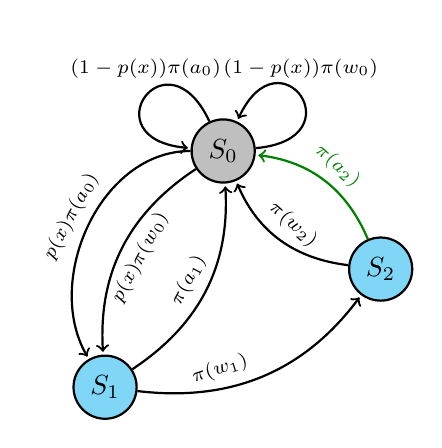
\begin{tikzpicture}[->,shorten >=1pt,auto,node distance=3cm,
            thick,main node/.style={circle,draw,font=\sffamily\Large\bfseries}]

        \node[fill=gray!50, circle, draw=black] (0) at (0,0) {$S_0$};
        \node[fill=cyan!50, circle, draw=black] (1) at (-1.5,-3) {$S_1$};
        \node[fill=cyan!50, circle, draw=black] (2) at (2,-1.5) {$S_2$};

        \path[every node/.style={font=\sffamily\scriptsize}]
        (0) edge [in=175,out=115, loop] node[above=3pt] {$(1-p(x)) \pi(a_0)$} (0)
        (0) edge [in=65,out=5, loop] node[above=3pt] {$(1-p(x)) \pi(w_0)$} (0)
        (0) edge [in=120,out=180] node[above, rotate=62] {$p(x) \pi(a_0)$} (1)
        (0) edge [bend right] node[below, rotate=62] {$p(x) \pi(w_0)$} (1)
        (1) edge [bend right] node[above, rotate=62] {$\pi(a_1)$} (0)
        (1) edge [bend right] node[rotate=18] {$\pi(w_1)$} (2)
        (2) edge [bend left] node[above, rotate=-42] {$\pi(w_2)$} (0)
        (2) edge [bend right, black!50!green] node[above, rotate=-42] {$\pi(a_2)$} (0);

    \end{tikzpicture}
    \caption{\label{fig:delayed_mdp} Graph showing the delayed action MDP}
\end{figure}

% reduced markov processes of observations
\begin{figure}[H]
    \centering
    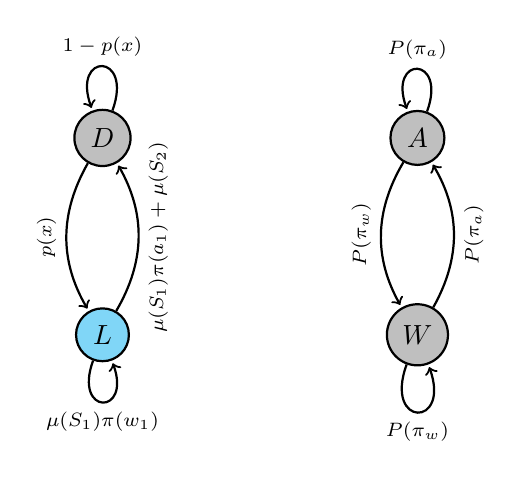
\begin{tikzpicture}[->,shorten >=1pt,auto,node distance=3cm,
            thick,main node/.style={circle,draw,font=\sffamily\Large\bfseries}]

        \node[fill=gray!50, circle, draw=black] (D) at (4,0) {$D$};
        \node[fill=cyan!50, circle, draw=black] (L) at (4,-2.5) {$L$};
        \node[fill=gray!50, circle, draw=black] (A) at (8,0) {$A$};
        \node[fill=gray!50, circle, draw=black] (W) at (8,-2.5) {$W$};

        \path[every node/.style={font=\sffamily\scriptsize}]
        (D) edge [in=110,out=70, loop] node[above] {$1-p(x)$} (D)
        (D) edge [bend right] node[above, rotate=90] {$p(x)$} (L)
        (L) edge [bend right] node[below, rotate=90] {$\mu(S_1)\pi(a_1) + \mu(S_2)$} (D)
        (L) edge [in=290,out=250, loop] node[below] {$\mu(S_1)\pi(w_1)$} (L)
        (A) edge [in=110,out=70, loop] node[above] {$P(\pi_a)$} (A)
        (A) edge [bend right] node[above, rotate=90] {$P(\pi_w)$} (W)
        (W) edge [bend right] node[below, rotate=90] {$P(\pi_a)$} (A)
        (W) edge [in=290,out=250, loop] node[below] {$P(\pi_w)$} (W);

    \end{tikzpicture}
    \caption{\label{fig:reduced_mps} Reduced models for Observation of light (left) and action (right).}
\end{figure}


\begin{figure}[H]
    \centering
    % L=2 light process
    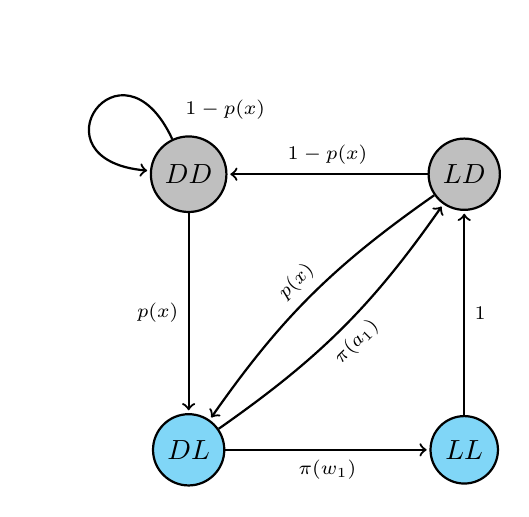
\begin{tikzpicture}[->,shorten >=1pt,auto,node distance=3cm,
            thick,main node/.style={circle,draw,font=\sffamily\Large\bfseries}]

        \node[fill=gray!50, circle, draw=black] (DD) at (0,3.5) {$DD$};
        \node[fill=gray!50, circle, draw=black] (LD) at (3.5,3.5) {$LD$};
        \node[fill=cyan!50, circle, draw=black] (DL) at (0,0) {$DL$};
        \node[fill=cyan!50, circle, draw=black] (LL) at (3.5,0) {$LL$};

        \path[every node/.style={font=\sffamily\scriptsize}]
        (DD) edge [in=175,out=115, loop] node[right=1cm] {$1-p(x)$} (DD)
        (DD) edge node[left] {$p(x)$} (DL)
        (DL) edge [bend right=10]  node[below, rotate=45] {$\pi(a_1)$} (LD)
        (LD) edge [bend right=10]  node[above, rotate=45] {$p(x)$} (DL)
        (LD) edge node[above] {$1-p(x)$} (DD)
        (DL) edge node[below] {$\pi(w_1)$} (LL)
        (LL) edge node[right] {$1$} (LD);

    \end{tikzpicture}
    \caption{\label{fig:mp1_L2} Internal model with sufficient complexity.}
\end{figure}

\section{Results} \label{sec:results}

\begin{figure}[H]
    \centering
    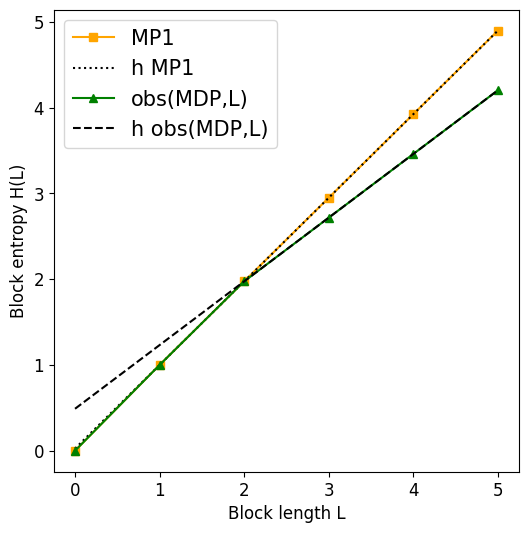
\includegraphics[width=0.5\linewidth]{../figures/mp1_vs_obsL.png}
    \caption{\label{fig:mp1_vs_obsL} Plot showing the difference between MP1 and the MDP.}
\end{figure}

Talk about behaviour correlating to order 2 of process, in agreement with Crutchfield.
Also do the same plot for MP2 and action as well, showing hidden Markov convergence.

\newpage
\begin{figure}[H]
    \centering
    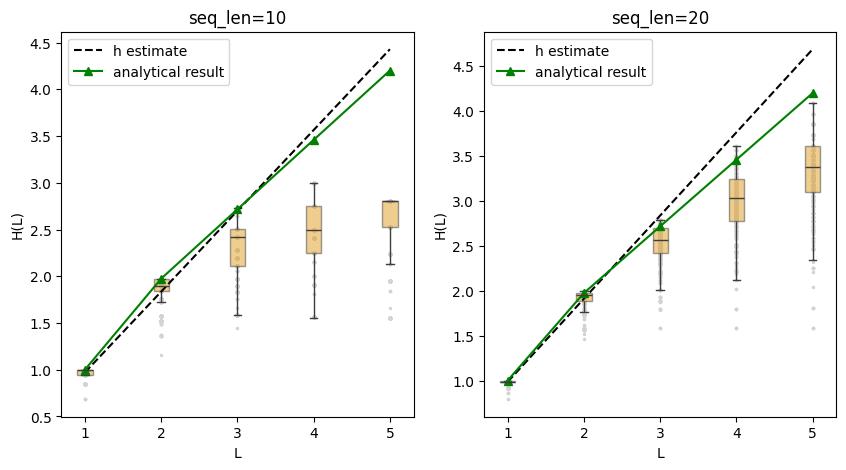
\includegraphics[width=1\linewidth]{../figures/block_entropy_estimation.png}
    \caption{\label{fig:entropy_est} Plot showing the bias and variance of the plug in estimator for block Entropy.}
\end{figure}

$$\hat{H}(s^L) = -\sum_i \frac{n_i}{N} \log_2{\frac{n_i}{N}}$$

(Lesne et al.) (10.1103/PhysRevE.79.046208) Entropy estimation of short (time correlated) sequences
Upper bound on block length given a sequence of observations, in order to have good estimates:
$$ n \leq \frac{N h_\mu}{\ln(k)} $$

with word length $n$, length of observation sequence $N$ and number of symbols $k$.

They propose first estimating the entropy rate using Lempel-Ziv complexity(iterative algorithm moving through sequence), then setting the sequence length/word length accordingly.

$$ \hat{L}_0 = \frac{\mathcal{N}_w \ln(N)}{N},\ \hat{L}=\frac{\mathcal{N}_w[1+\log_k\mathcal{N}_w]}{N},\ \lim_{n \to \infty}\hat{L} = \frac{h_\mu}{\ln(k)} $$

With $N$ the length of the observation sequence and $\mathcal{N}_w$ parsed words from the Lempel-Ziv algorithm.
For the plug in estimator, error bars are computable, meaning computable confidence intervals.

Larson et al. (10.1016/j.procs.2011.04.172) use
$$ \mathcal{L} h_\mu \geq L|A|^L \ln|A| $$
solving for $L$ given $\mathcal{L}$ returns $W(\mathcal{L} h_\mu) / \ln|A|$ (mathematica), with the Lambert $W$ function.
(gives better estimate)

\begin{figure}
    \centering
    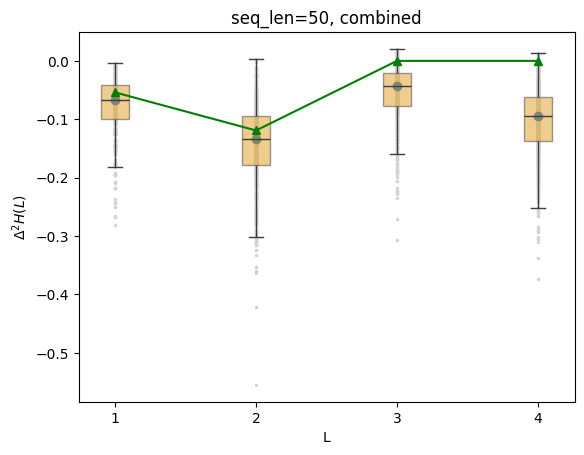
\includegraphics[width=0.5\linewidth]{../figures/predictability_gain_estimation.png}
\end{figure}

\begin{figure}
    \centering
    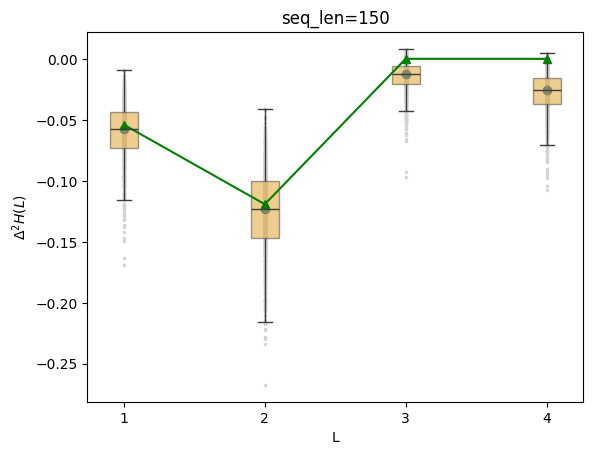
\includegraphics[width=0.5\linewidth]{../figures/predictability_gain_estimation_optimal.png}
\end{figure}

deviation from analytical:
[-0.00365034217876947 -0.00365907607011157 -0.0124851947847702
-0.0251811425394552]

\section{Conclusion} \label{sec:conclusion}


\section{Acknowledgements} \label{sec:acknowledgements}


\clearpage
\section*{Declaration of Authorship}

I hereby solemnly declare, by my own signature, that I have independently authored the presented work and have not used any sources or aids other than those indicated. All passages taken verbatim or in content from the specified sources are identified as such.

I consent to the archiving of this Bachelor thesis.

\hfill
\vspace{2cm} Innsbruck, \findate \hfill Lukas Prader \includegraphics[height = 10mm]{"signature.png"}


\newpage
\printbibliography[]
\newpage
\appendix



\end{document}